\documentclass[10pt]{article}
\usepackage{lscape}
\usepackage{geometry}
\usepackage{graphicx} % Necessario per scalare la tabella
\usepackage{adjustbox} % Opzionale, per un controllo più fine della dimensione
\usepackage{array}
\usepackage{amsmath}
\usepackage{amssymb}

\geometry{a4paper, left=0.5cm, right=1cm, top=1cm, bottom=1cm}

\pagestyle{empty}

\graphicspath{{img/}}

\let\olditemize\itemize
\renewcommand\itemize{\olditemize\setlength\itemsep{0em}}

\begin{document}
\begin{landscape}

% Posizionamento della tabella in modo fisso e ridotto
\begin{picture}(0,0)
    \put(585,-535){ % Coordina verticalmente e orizzontalmente la posizione della tabella
        \scalebox{0.7}{ % Riduce la tabella al 70% della sua dimensione originale
        \begin{tabular}{|c c c c c|}
        \hline
        $\sqrt{1}=1$ & $\sqrt{4}=2$ & $\sqrt{9}=3$ & $\sqrt{16}=4$ & $\sqrt{25}=5$ \\
        $\sqrt{36}=6$ & $\sqrt{49}=7$ & $\sqrt{64}=8$ & $\sqrt{81}=9$ & $\sqrt{100}=10$\\
        $\sqrt{121}=11$ & $\sqrt{144}=12$ & $\sqrt{169}=13$ & $\sqrt{196}=14$ & $\sqrt{225}=15$ \\ 
        $\sqrt{256}=16$ & $\sqrt{289}=17$ & $\sqrt{324}=18$ & $\sqrt{361}=19$ & $\sqrt{400}=20$\\
        $\sqrt{441}=21$ & $\sqrt{484}=22$ & $\sqrt{529}=23$ & $\sqrt{576}=24$ & $\sqrt{625}=25$ \\ 
        $\sqrt{676}=26$ & $\sqrt{729}=27$ & $\sqrt{784}=28$ & $\sqrt{841}=29$ & $\sqrt{900}=30$\\
        \hline
        \end{tabular}
        }
    }
\end{picture}

% Testo normale qui
\noindent
\begin{minipage}[t]{0.49\textwidth}
\begin{tabular}{c}
    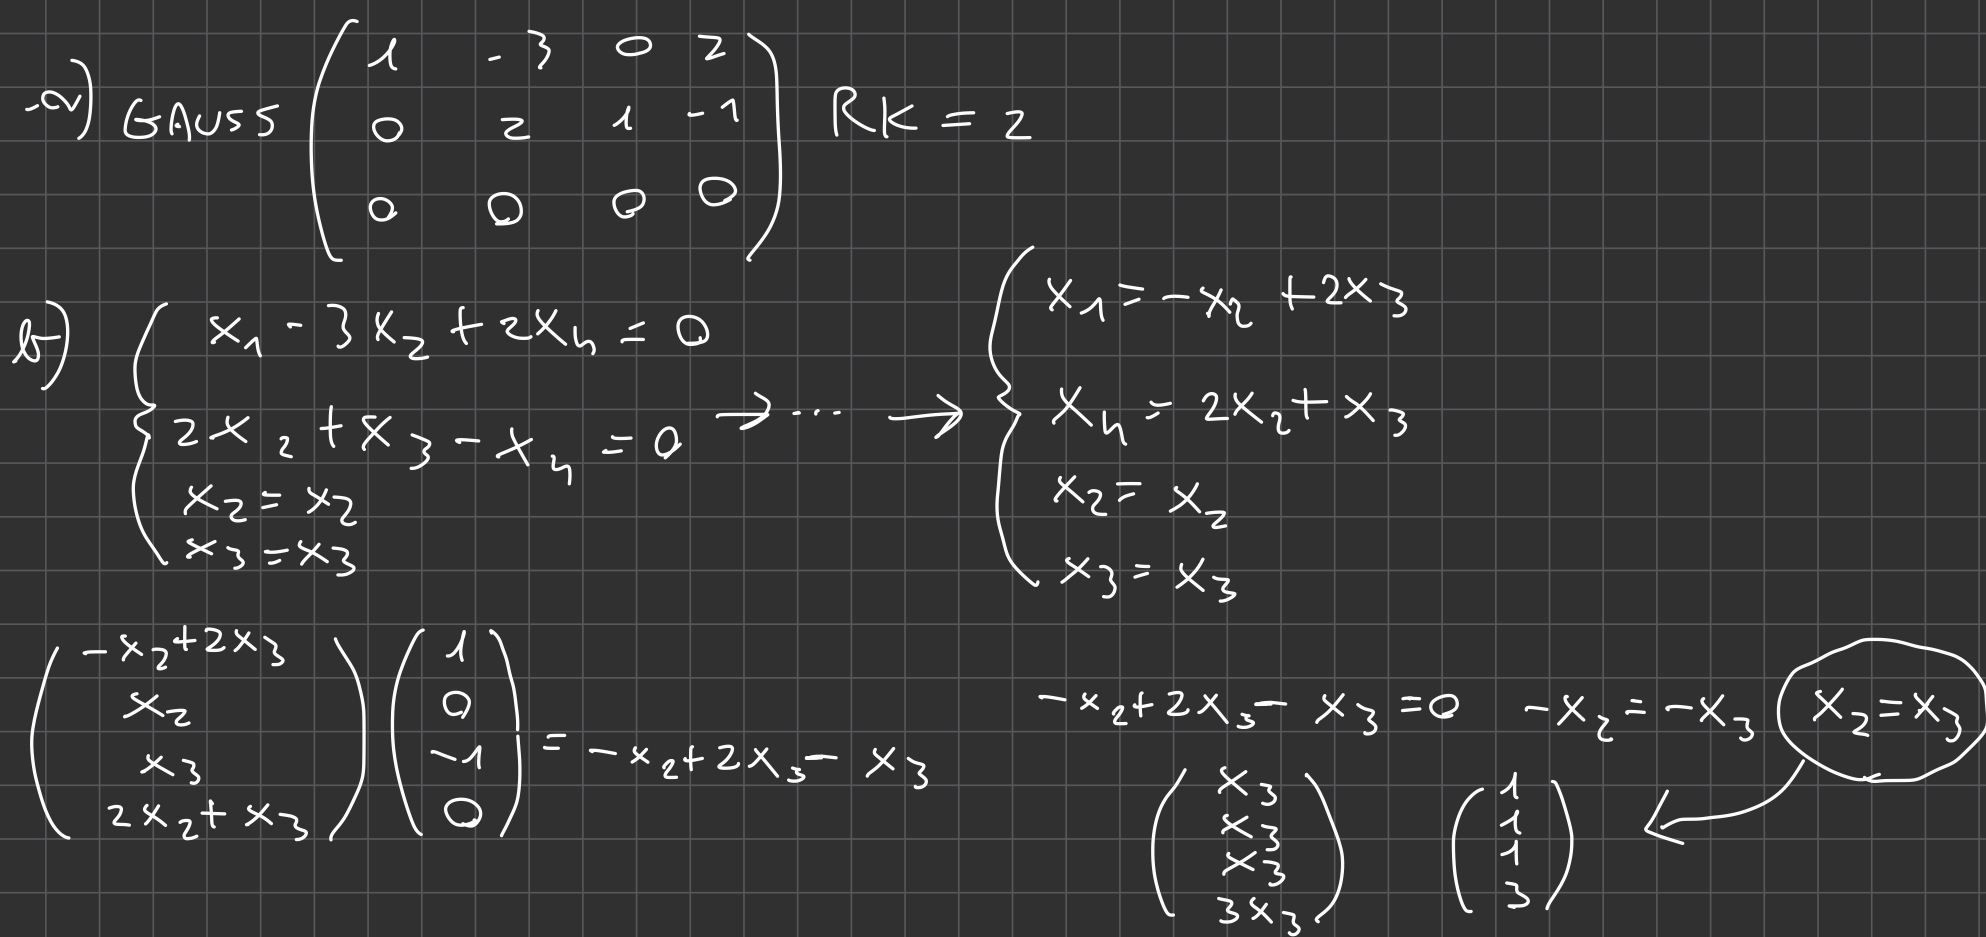
\includegraphics[scale=0.12]{es1.jpeg} \\ 
    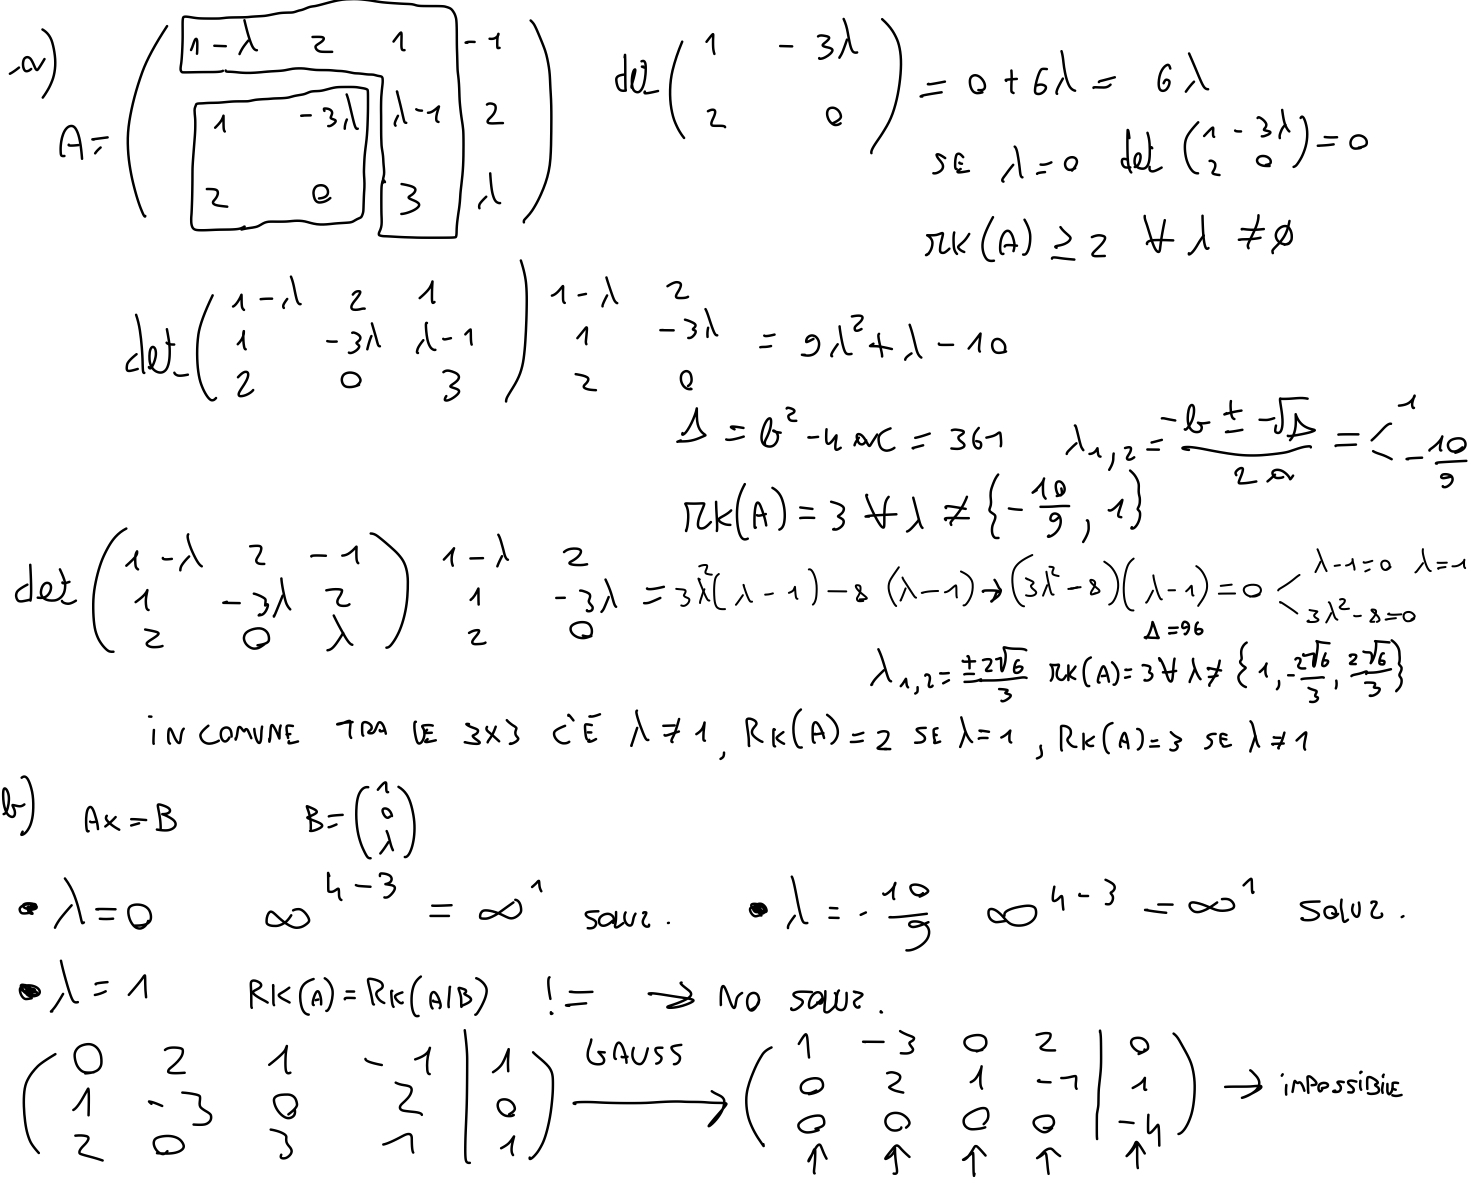
\includegraphics[scale=0.16]{es2.jpeg} \\
    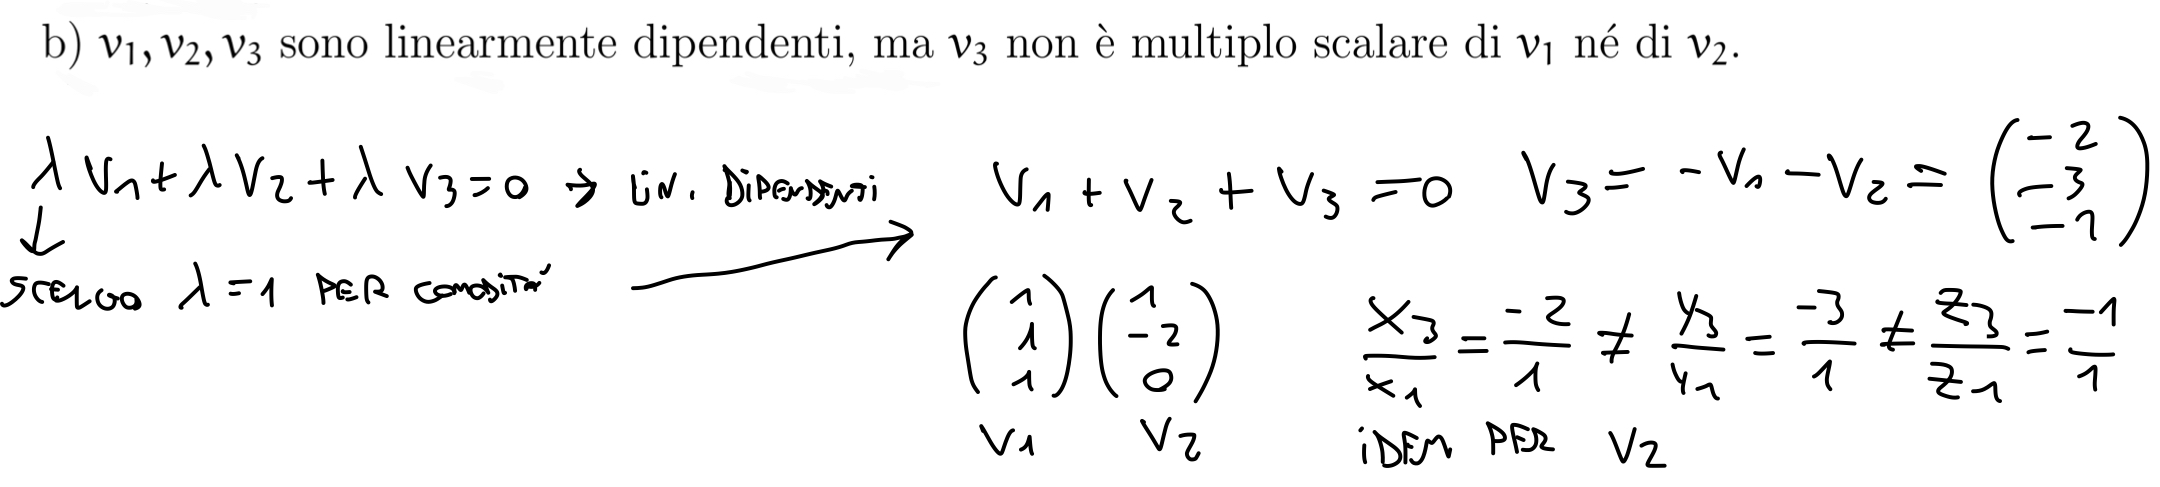
\includegraphics[scale=0.12]{es4.jpeg} \\
    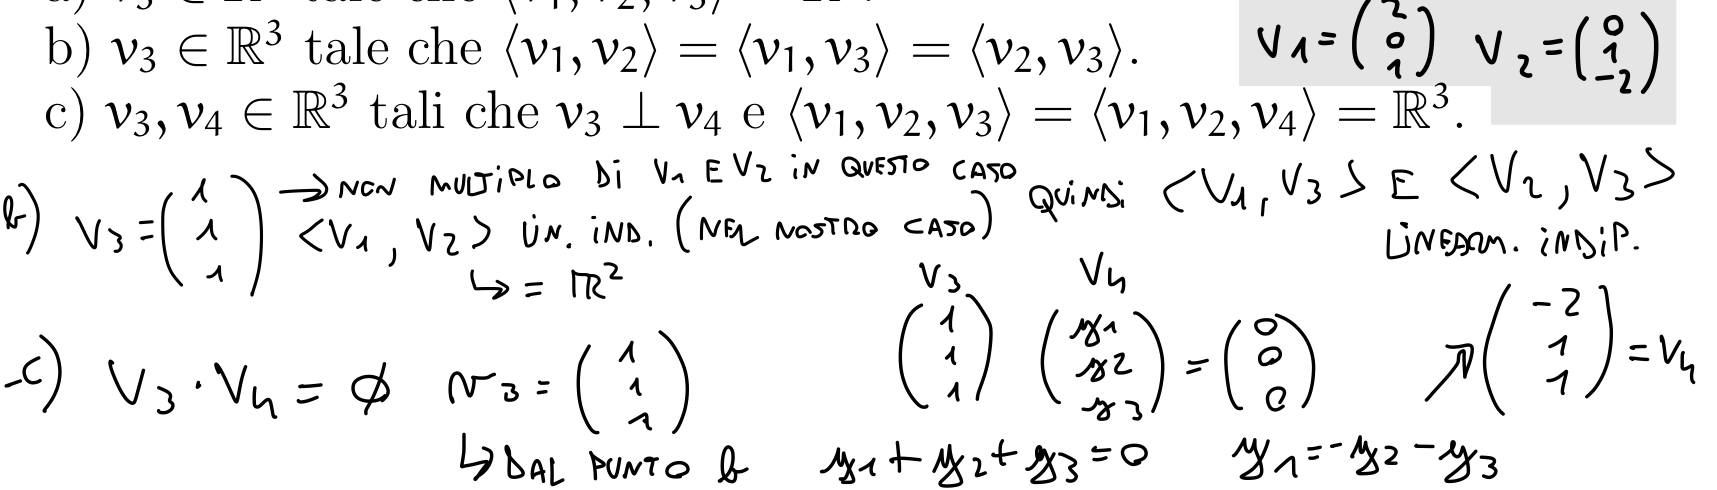
\includegraphics[scale=0.15]{es5.png} \\
\end{tabular}
\end{minipage}
%\hfill
\begin{minipage}[t]{0.49\textwidth}
    \tiny
\begin{picture}(0,0)
    \put(0,-10){
        \begin{tabular}{| m{1.2cm} | m{16.5cm} |}
            \hline
            Esercizio 1 & Fare Gauss per il rango, creare il sistema (prendo le x in comune e le tratto come libere), isolo le x, sostituisco le x trovate nel vettore X, eseguo $X\cdot v = 0$, isolo una x, sostituisco nuovamente e poi costruisco il vettore prendendo i coefficienti\\
            \hline
            Esercizio 2 & Calcolare il det di una $2\times2$ a caso, se det $\neq 0$ allora $rk(A)\geq 2$ possiamo orlarla, altrimenti ne cerco un'altra, calcoliamo il det di tutte le possibili $3\times3$, le $\lambda$ in comune alle $3\times3$ sono quelle che rk(A)=2, tutte le altre rk(A)=3; \\
            \hline
            Esercizio 3 & \begin{itemize}
                \item Se $A$ è una matrice nilpotente (ossia esiste un intero positivo $n$ tale che $A^{n}=0$) allora $\det A=0$ $\rightarrow$ Nilpotente non invertibile allora $\det A=0$
                \item Se $A$ è una matrice simmetrica, allora $A^{2}$ è simmetrica $\rightarrow$ $M$ simmetrica se $M=M^{T}\Rightarrow M^{T}\cdot M^{T}=(M\cdot M)^{T}\Rightarrow M = M^{T}$, sostituisci $M$ con $A^{2}$
                \item Sia $A\in M_{3,2}(\mathbb{R})$ di rango 2, allora il sistema lineare $AX=B$ ammette soluzioni comunque si scelga la matrice $B$ dei termini noti. $\rightarrow$ Se si sceglie $B$ t.c $rk(A|B)=3$ allora il sistema è impossibile (non ammette soluzioni) per Rouché-Capelli ($\infty^{2-3}$)
                \item $A^{3}-A=I_{2}\rightarrow A(A^{2}-I)=I\Rightarrow(A^{2}-I)=A^{-1}$ quindi $AA^{-1}=I$ ($A$ è invertibile)
                \item $A^{3}-A=0\rightarrow A(A^{2}-I)=0\Rightarrow A=0, A^{2}-I=0\Rightarrow A=0, A^{2}=I$ quindi $A$ è invertibile se $A^{2}=I$ altrimenti se $A=0$ non è invertibile
                \item $A^{3}-A=\begin{pmatrix}
                    1 & 1 \\
                    2 & 3
                \end{pmatrix}\rightarrow A(A^{2}-I)=\begin{pmatrix}
                    1 & 1 \\
                    2 & 3
                \end{pmatrix}\Rightarrow A=\begin{pmatrix}
                    1 & 1 \\
                    2 & 3
                \end{pmatrix}, A^{2}-I=\begin{pmatrix}
                    1 & 1 \\
                    2 & 3
                \end{pmatrix}\Rightarrow A^{2}=\begin{pmatrix}
                    1 & 1 \\
                    2 & 3
                \end{pmatrix}+I=\begin{pmatrix}
                    2 & 1 \\
                    2 & 4
                \end{pmatrix}\Rightarrow A=\begin{pmatrix}
                    \sqrt{2} & 1 \\
                    \sqrt{2} & 2
                \end{pmatrix}$ poi calcolo il determinante delle due $A$ e uso il teorema di Binét: $\det\begin{pmatrix}
                    1 & 1 \\
                    2 & 3
                \end{pmatrix}=1, \det\begin{pmatrix}
                    \sqrt{2} & 1 \\
                    \sqrt{2} & 2
                \end{pmatrix}=2\sqrt{2}-\sqrt{2}\neq 0$, quindi $A$ è invertibile
                \item $A$ è invertibile, allora $\det(A)>0\rightarrow$ Falso, per Binét $A$ è invertibile se $\det A\neq 0$ (quindi può essere anche negativo).
                \item Se $A$ è $B$ sono invertibili, $AB$ è invertibile $\rightarrow$ Vero, $AB$ è invertibile se $\det(AB)\neq 0$ e per Binét $\det(AB)=\det A \cdot \det B\neq 0$
                \item Se $A^{13}=B$ e $B$ è invertibile, allora $A$ è invertibile $\rightarrow$ Vero, $\det(A^{13})=\det(B)\Rightarrow \det(A)^{13}=\det(B)$ sappiamo che $\det(B)\neq 0$ quindi $\det(A)\neq 0$ e quindi $A$ è invertibile
                \item I vettori colonna di $A\in M_{n}(\mathbb{R})$ generano $\mathbb{R}^{n}\rightarrow$ $A$ è invertibile perchè visto che i vettori sono base di $\mathbb{R}^{n}$ allora la matrice ha rango $n$(massimo) e quindi è invertibile
                \item Se $A\in M_{3,4}(\mathbb{R})$ ha due minori distinti di ordine 3 con determinante nullo, $\text{rk}(A)<3$ $\rightarrow$ vero, sappiamo che esistono solo due sottomatrici $3\times 3$ quindi se entrambe hanno determinante nullo allora $\text{rk}(A)<3$
                \item Tre vettori qualsiasi di $\mathbb{R}^{2}$ sono linearmente dipendenti $\rightarrow$ Usiamo la regola per essere base di $R^{N}$ che dice che sono linearmente indipendenti se il rango della matrice composta dai vettori è $N$, quindi basta trovare un vettore per cui il rango non è 2 per avere i vettori linearmente dipendenti  
            \end{itemize}\\
            \hline
            Esercizio 4 & \begin{itemize}
                \item I vettori $v_{1},\ldots ,v_{n}$ sono base di $R^{N}$ se $\text{rk}(M)=N$ con $M=(v_{1}\ldots v_{n})$ (M matrice composta dai vettori)
                \item Base ortogonale di $v,w$: $\begin{pmatrix}
                    \det(R_{2}R_{3}) \\
                    -\det(R_{1}R_{3}) \\
                    \det(R_{1}R_{2})
                \end{pmatrix}$, $R_{i}$ sono le righe dei vettori. $v,w$ devono essere ortogonali 
                \item Dipendenza lineare: $\alpha v_{1}+\beta v_{2} +\ldots + kv_{n} = 0$ oppure la matrice composta dai vettori non ha rango $N$
                \item Indipendenza lineare: $\alpha v_{1}+\beta v_{2}+\ldots+ kv_{n} = 0 \rightarrow \alpha = \beta = 0$ oppure la matrice composta dai vettori ha rango $N$
                \item $v_{3}=\begin{pmatrix}
                    x_{3} \\ y_{3} \\ z_{3}
                \end{pmatrix}$ è multiplo scalare di $v_{1}=\begin{pmatrix}
                    x_{1} \\ y_{1} \\ z_{1}
                \end{pmatrix}$ se $\frac{x_{3}}{x_{1}}=\frac{y_{3}}{y_{1}}=\frac{z_{3}}{z_{1}}=\alpha$
                \item Per "generare" $R^{N}$ i vettori combinati linearmente fanno ottenere qualsiasi vettore in $R^{N}$. Gli N vettori in questione devono essere linearmente indipendenti.
                \item $v_{2} \notin \langle v_{1} \rangle$ significa che $v_{2}$ non appartiene allo spazio generato da $v_{1}$ e quindi $v_{2}$ non deve essere multiplo scalare di $v_{1}$
                \item Due vettori $v_1$ e $v_2$ sono ortogonali ($v_{1}\bot v_{2}$) tra loro quando il loro prodotto scalare e' 0
                \item Norma vettore $||v|| = \sqrt{v_{1}^{2} + v_{2}^{2}}$, per "allungare" un vettore a una lunghezza L si usa la formula $v' = L\cdot \frac{1}{||v||}\cdot v$
            \end{itemize}\\
            \hline
            &  \begin{itemize}
                \item Gauss: $R_{i}=R_{i}+\left(\frac{-a_{ij}}{a_{jj}}\right)\cdot R_{j}$
                \item Rouché-Capelli: $\infty^{\#incognite-\text{rk}(A)}$
                \item A invertibile se $\det A \neq 0$, $\det (A^{-1})=\frac{1}{\det A}$
                \item $A$ non invertibile se $A^{N}=0$
                \item Il prodotto di due matrici diagonali è diagonale, una matrice diagonale non è per forza invertibile (potrebbe avere degli zeri nella diagonale) e ogni matrice diagonale è simmetrica
                \item Teorema di Binét: $\det(AB)=\det A \cdot \det B$
                \item Calcolo matrice inversa: scriviamo $(M|I)$, eseguiamo Gauss (da entrambe le parti), gli elementi sopra il pivot li poniamo tutti a 0 (sempre alla Gauss dal basso verso l'alto), otteniamo $(I|M^{-1})$
                \item Prodotto scalare: $\begin{pmatrix}
                    x_{1} \\ y_{1} \\ z_{1}
                \end{pmatrix}\cdot \begin{pmatrix}
                    x_{2} \\ y_{2} \\ z_{2}
                \end{pmatrix}=x_{1}x_{2}+y_{1}y_{2}+z_{1}z_{2}$
                \item $AX=B$ ammette soluzioni se $\text{rk}(A|B)=\text{rk}(A)$
            \end{itemize}\\
            \hline
        \end{tabular}
    }
\end{picture}

\end{minipage}

\end{landscape}
\end{document}
